\documentclass[12pt]{article}

\usepackage{graphicx}
\usepackage[margin = 3 cm]{geometry}
\usepackage[english]{babel}
\usepackage[utf8x]{inputenc}
\usepackage{amsmath}
\usepackage[colorinlistoftodos]{todonotes}
\usepackage{listings}
\usepackage{float} %For image positioning
\usepackage{subcaption} %For even more image positioning
\usepackage[figurename=Fig.]{caption}
\usepackage{rotating}





\begin{document}
%%Forside



\begin{titlepage}

\newcommand{\HRule}{\rule{\linewidth}{0.5mm}} % Defines a new command for the horizontal lines, change thickness here

\center % Center everything on the page
 
%----------------------------------------------------------------------------------------
%	HEADING SECTIONS
%----------------------------------------------------------------------------------------

\textsc{\LARGE Aalborg Tekniske Gymnasium}\\[1.5cm] % Name of your university/college
\textsc{\Large P4 - El-Tek}\\[0.5cm] % Major heading such as course name
\textsc{\large El-teknik A}\\[0.5cm] % Minor heading such as course title

%----------------------------------------------------------------------------------------
%	TITLE SECTION
%----------------------------------------------------------------------------------------

\HRule \\[0.4cm]
{ \huge \bfseries En fjernstyret kanon  }\\[0.4cm] % Title of your document
\HRule \\[1.5cm]
 
%----------------------------------------------------------------------------------------
%	AUTHOR SECTION
%----------------------------------------------------------------------------------------

\begin{minipage}{0.4\textwidth}
\begin{flushleft} \large
\emph{Forfatter:}\\
Nikolai \textsc{Bonderup}\\ % Your name
Sebastian \textsc{Lassen}\\
Lucas \textsc{Rasmussen}
\end{flushleft}
\end{minipage}
~
\begin{minipage}{0.4\textwidth}
\begin{flushright} \large
\emph{Vejleder:} \\
Pia \textsc{Thomsen} \\ % Supervisor's Name
Tom \textsc{Berthelsen}\\
\end{flushright}
\end{minipage}\\[2cm]

% If you don't want a supervisor, uncomment the two lines below and remove the section above
%\Large \emph{Author:}\\
%John \textsc{Smith}\\[3cm] % Your name

%----------------------------------------------------------------------------------------
%	DATE SECTION
%----------------------------------------------------------------------------------------

{\large \today}\\[2cm] % Date, change the \today to a set date if you want to be precise



\vfill % Fill the rest of the page with whitespace

\end{titlepage}



%%%%---------------------------------------------
%%Titelblad
%%%%---------------------------------------------
\section*{Titelblad}
{\large \textbf{Projekttitel}} Sensorer og datakommunikation\\[0.5cm]
{\large \textbf{Uddannelsessted og klasse}} Aalborg tekniske Gymnasium, Q16\\[0.5cm]
{\large \textbf{Fag}} Teknikfag, Elektronik A\\[0.5cm]
{\large \textbf{Projektperiode}} x/x/2018 - 6/2/2019\\[0.5cm]
{\large \textbf{Projektet udarbejdet af:}}\\[2cm]

\rule{0.5\textwidth}{0.4pt}\\
\textbf{Lucas Mark Rasmussen} \\[1cm]

\rule{0.5\textwidth}{0.4pt}\\
\textbf{Sebastian Lassen} \\[1cm]

\rule{0.5\textwidth}{0.4pt}\\
\textbf{Nikolai Aaen Bonderup} \\[1cm]

\subsection*{Synopsis}
I dette projekt har vi fået til opgave at lave et produkt, som skal kunne opfylde nogle praktiske krav, der er givet ved en opgaveformulering og produktkrav. Der er blevet udleveret flere forskellige bluetooth elementer, hvorefter gruppen selv har skulle idegenerere og konstruere et produkt som lever op til de krav, som er stillet i selve opgaveformuleringen (kravspecifikationen). Projektet har derfor resulteret i et kanontårn som kan kontrolleres trådløst og er i besiddelse af en form for interrupt, forskellige slags motorer og et mikrocontrollerprint.

\subsection*{Forord}
Rapporten består af otte hovedafsnit som er markeret i indholdsfortegnelsen og seks, hvis litteraturliste og bilag trækkes fra. Disse hovedafsnit har hver en mængde af underafsnit som også kan ses i selve indholdsfortegnelse. I afsnittene gennemgås arbejdet med robotten og overvejelser som gruppen har gjort sig. Der medfølger selvfølgelig billede af udvalgte dele af arbejdet, samt tekniske tegninger og i nogle tilfælde også tidligere versioner af disse tegninger for at vise en udvikling.

%%%%---------------------------------------------
%%Indholdsfortegnelse
%%%%---------------------------------------------
\newpage
\renewcommand{\contentsname}{Indholdsfortegnelse}
\tableofcontents
\newpage

%%%%---------------------------------------------
%%Begyndelse af rapport
%%%%---------------------------------------------

%%Indledning
\newpage
%Dokument til indledningen
\section{Indledning}

Projektet ligger under studieområdet, hvilket her betyder at vi skal kombinere vores teknikfag med et af vores studieretningsfag. Vi har i gruppen valgt at bruge Fysik A, da dette virkede som det mest oplagte valg ift. bidragelse med projektrelevant teori. Projektet skal derfor også overholde forskellige krav fra SO, el-tek og fysik A, som bliver yderligere fremhævet i kravspecifikationen.\\

Vi har i gruppen besluttet os for at bygge en fjernstyret airsoft kanon, da dette produkt vil tilfredsstille alle de givne el-tek krav, samt at fysikteorien omkring det skrå kast kan bruges til at bestemme, hvor dets projektil vil ramme og hvor hurtigt det bevæger sig. Det kan gøres ved at måle, hvor langt kanonen skyder og hvilken vinkel løbet er peget op med, for så derefter at beregne mundingshastigheden vha. formler for det skrå kast. Dette kan så krydstjekkes med en målt projektilhastighed for, at opnå et fysikeksperiment udført med hjælp af elektriske komponenter.


%%Kravspecifikation
\newpage
\documentclass[12pt]{article}

\usepackage{graphicx}
\usepackage[margin = 3 cm]{geometry}
\usepackage[english]{babel}
\usepackage[utf8x]{inputenc}
\usepackage{amsmath}
\usepackage[colorinlistoftodos]{todonotes}
\usepackage{listings}
\usepackage{float} %For image positioning
\usepackage{subcaption} %For even more image positioning
\usepackage[figurename=Fig.]{caption}
\usepackage{rotating}


\begin{document}

%%Problemanalyse
\newpage
%Dokument til Projektanalyse
\subsection{Projektanalyse}

I dette projekt skal vi kombinere Fysik A og el-tek til et SO forløb. I projektet er der flere faglige mål som skal opfyldes indenfor området el-tek og fysik. Selve opgaven lyder på at gøre brug af de elementer som er at finde under kravspecifikationer. I problemanalysen skal disse elementer altså gennemgås og der skal vurderes, hvilket et af dem bliver det største “problem” at arbejde med.\\

Det mest udfordrende bliver at få skabt kommunikation mellem selve kanonen og et kontrolelement. Der skal være en modtager og afsender, måske endda en af hver på både kontrolmodul og kanon-modulet alt efter hvor avanceret arbejdet med denne del af projektet skal være.\\

Et andet udfordrende problem bliver, hvordan selve lade- og affyringsmekanismen skal hænge sammen så den kan virke ved fjernstyring. Her skal flere forskellige typer motorer styres præcist gennem bluetooth.


%%Forside



\begin{titlepage}

\newcommand{\HRule}{\rule{\linewidth}{0.5mm}} % Defines a new command for the horizontal lines, change thickness here

\center % Center everything on the page
 
%----------------------------------------------------------------------------------------
%	HEADING SECTIONS
%----------------------------------------------------------------------------------------

\textsc{\LARGE Aalborg Tekniske Gymnasium}\\[1.5cm] % Name of your university/college
\textsc{\Large Studieområde-projekt}\\[0.5cm] % Major heading such as course name
\textsc{\large Fysik A \& el-teknik A}\\[0.5cm] % Minor heading such as course title

%----------------------------------------------------------------------------------------
%	TITLE SECTION
%----------------------------------------------------------------------------------------

\HRule \\[0.4cm]
{ \huge \bfseries En fjernstyret kanon \& det skrå kast  }\\[0.4cm] % Title of your document
\HRule \\[1.5cm]
 
%----------------------------------------------------------------------------------------
%	AUTHOR SECTION
%----------------------------------------------------------------------------------------

\begin{minipage}{0.4\textwidth}
\begin{flushleft} \large
\emph{Forfatter:}\\
Nikolai \textsc{Bonderup}\\ % Your name
Sebastian \textsc{Lassen}\\
Lucas \textsc{Rasmussen}
\end{flushleft}
\end{minipage}
~
\begin{minipage}{0.4\textwidth}
\begin{flushright} \large
\emph{Vejleder:} \\
Pia \textsc{Thomsen} \\ % Supervisor's Name
Tom \textsc{Berthelsen}\\
\end{flushright}
\end{minipage}\\[2cm]

% If you don't want a supervisor, uncomment the two lines below and remove the section above
%\Large \emph{Author:}\\
%John \textsc{Smith}\\[3cm] % Your name

%----------------------------------------------------------------------------------------
%	DATE SECTION
%----------------------------------------------------------------------------------------

{\large \today}\\[2cm] % Date, change the \today to a set date if you want to be precise



\vfill % Fill the rest of the page with whitespace

\end{titlepage}



%%Problemformulering
\newpage
%Dokument til Projektformulering
\section{Projektformulering}

%%Problemformulering
\newpage
%Dokument til projektafgrænsningen
\section{Projektafgrænsning}

Vi har planlagt at arbejde med en kanon som skal kunne rotere 360 grader, samt have et vinkelinterval til affyring af kanonen på mindst 100 grader. Den fjernstyrede kanon skal være i stand til at modtage information fra et kontrolmodul. Dette skal ske ved brug af en bluetooth enhed eller et andet trådløst kommunikationsmodul. Der skal altså laves en mikrocontroller som kan styre kanonen gennem disse trådløse moduler ved at få kommandoer fra et kontrolmodul.\\

\begin{figure}[H]
\centering
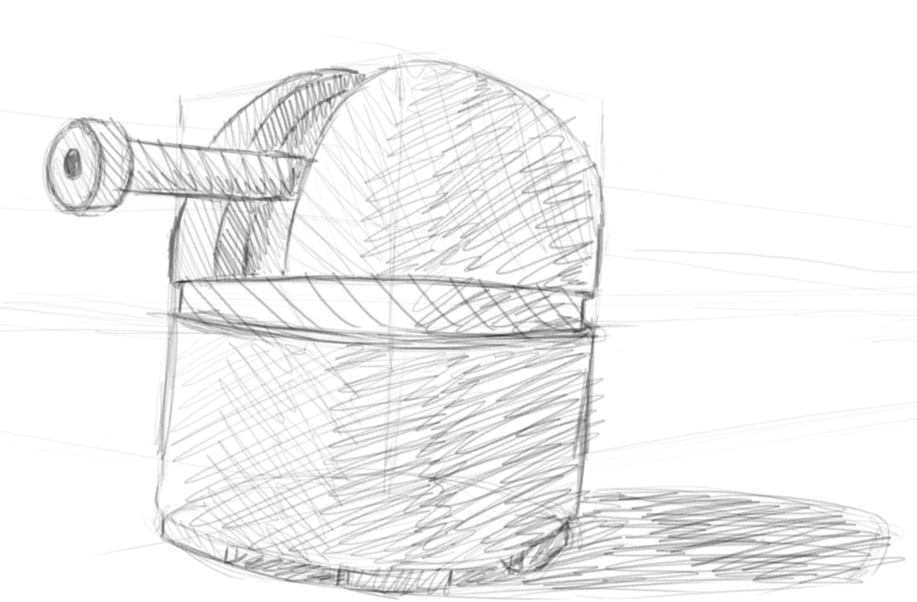
\includegraphics[scale=0.4]{Billeder/Koncept_turret.png}
\caption{Koncept af kanon.}
\label{fig:KonceptKanon}
\end{figure}

Selve kanons affyringsmekanisme laves enten med en “airsoft” pneumatisk gearkasse, hvor en DC motor bruges til at trække en fjeder op. Denne fjeder laver et lufttryk i gearkassens trykkammer som kan bruges til at skyde et projektil afsted. Selve robottens krop laves vha. 3D print af de enkelte komponenter, der sættes sammen med enten lim eller skruer. \\

Til udarbejdningen af det fysikvidenskabelige dokumentation kan der påmonteres forskellige accelerometerer, som kan bruges til at bestemme skydevinklen. Derudover kan der alternativt måles, hvor langt projektilet bliver affyret for så, at kunne beregne dets hastighed, hvis affyringsvinklen er kendt.

\begin{figure}[H]
\centering
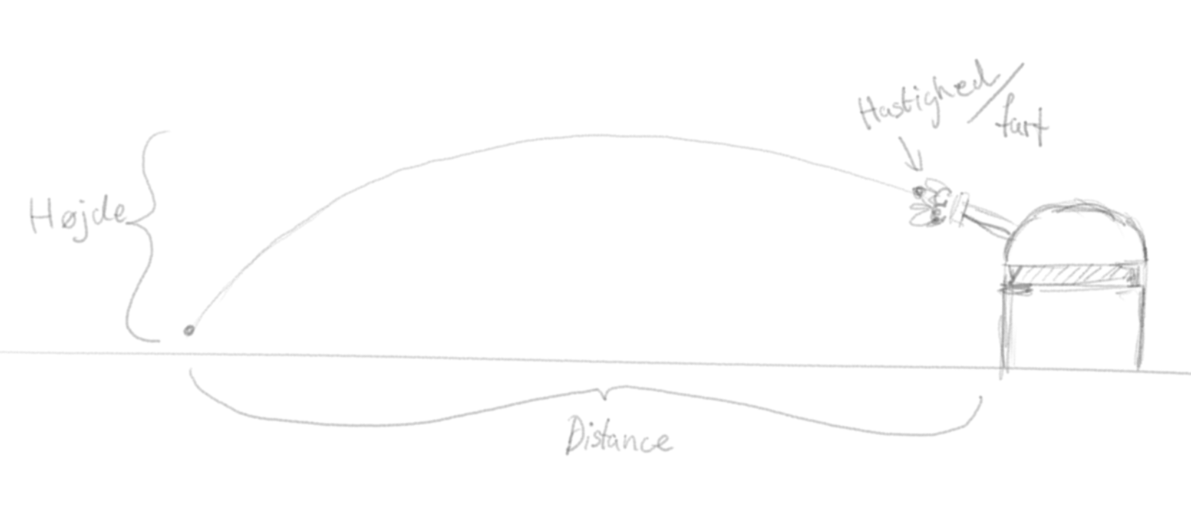
\includegraphics[scale=0.4]{Billeder/Fysik_koncept.png}
\caption{Fysik relevant til kanonen.}
\label{fig:FysikKoncept}
\end{figure}

%%Kravspecifikation
\newpage
%Dokument til kravspecifikationer
\section{kravspecifikationer}

De opstillede krav fra el-tek:

Der skal bruges en “interrupt” (HW - Kontakt, SW - Timer).
Der skal altså i projektet bruges enten en kontakt eller timer i vores kredsløb. Det er påkrævet at denne har en relevant betydning for selve kredsløbet og ikke har en meningsløs funktion.

Der skal være et sensor input: analog til digital konvertering.
Dette forstås som at der skal bruges en type sensor, som måler noget analogt, der derefter kan oversættes til noget digitalt vha. en mikroprocessor. Dette kunne for eksempel være en afstandssensor.

Digital til Analog konvertering.
Dette vil ved brug af Arduino i de fleste tilfælde være at bruge et PWM signal til kontrol af et elektronisk element.

Der skal bruges datakommunikation (til pc, viserinstrument eller trådløst element).
Dette ville være en form for input/output type af kontrol i forhold til vores produkt. Her skal gruppen kunne give en eller anden form for ordre til produktet og produktet skal så udføre en bestemt handling. Dette kunne opfyldes ved at styre kanonens vinkel med en controller vha. bluetooth.

Et print til en mikrocontroller.
Der skal til produktet bruges et selvproduceret mikrocontrollerprint. Denne microcontroller skal kunne styre en af hovedelementerne i selve produktet for at opfylde kravet om at have en relevant funktion.

Udover de specifikke krav skal der også indrages relevant fysikteoretisk arbejde, som udmunder i afleveringen af videnskabelig dokumentation vedrørende det valgte fysikteori og el-tek produkt.


\end{document}

\newpage
\section{Systembeskrivelse}
Afsnitet systembeskrivelse beskriver de forskellige elektroniske komponenters relation til hinanden via.Til hvert elektriske kredsløb er der et blokdiagram og en uddybende forklaring af blokdiagrammets elementer. Derudover er der et flowdiagram som viser det elektriske kredsløbs funktion.\\

I dette projekt er der i alt 2 forskellige elektriske kredsløb ( hvis man ignorere de isoleret kredsløb, som bliver skabt pga. Brugen af H-broer og hardball pistol). Kredsløb \#1 er kredsløbet som kan findes på selve kanon. Dette kredsløb styrer kanonens bevægelse vha. Motorer og sensorer. Kredsløb \#2 er kredsløbet som findes på kontrolleren. Dette kredsløb bruges til at styrer kanonen gennem et bluetooth signal fra kredsløb \#2 til kredsløb \#1. \\

%Kredsløb 1
\subsection{Kanontårn}

\begin{figure}[H]
\centering
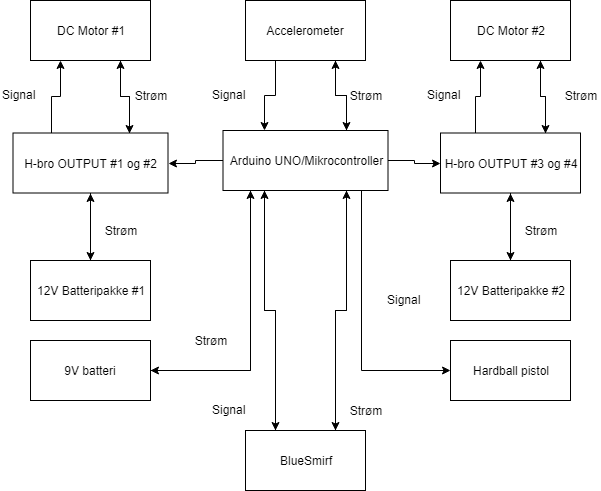
\includegraphics[scale=0.8]{Billeder/Kredsloeb1.png}
\caption{Blokdiagram af kanontaarnets elektriske kredslob.}
\label{fig:Blokdiagram1}
\end{figure}


\begin{figure}[H]
\centering
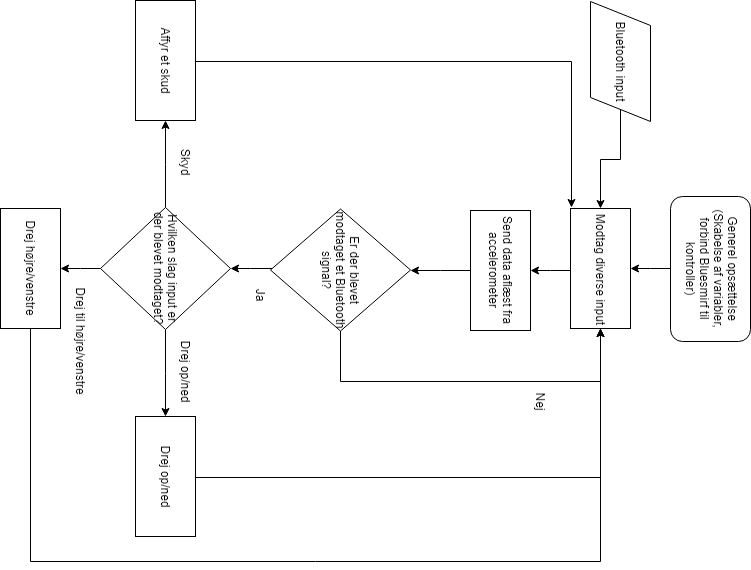
\includegraphics[scale=0.8]{Billeder/Flowchart1.png}
\caption{Flowdiagram af kanontaarnets funktion.}
\label{fig:Flowdiagram1}
\end{figure}

\newpage
\textbf{Systemdele}

%Liste
\begin{itemize}
	\item Arduino UNO / Mikrocontroller
\begin{itemize}
\item På blokdiagrammet kan det ses, at Arduinoen er forbundet til næsten alle elektroniske elementer i kanontårnet. I arduinoens sted kan gruppens egen mikrocontroller print også monteres, da den har samme funktionalitet.
\end{itemize}

	\item 9V batteri
\begin{itemize}
\item Dette 9 volts batteri fungere som Arduinoens / mikrocontrollerens strømforsyning.
\end{itemize}

	\item 6V batteripakke \#1
\begin{itemize}
\item Denne batteripakke fungere som motor \#1’s strømforsyning.
\end{itemize}

	\item 6V batteripakke \#2
\begin{itemize}
\item Denne batteripakke fungere som motor \#2’s strømforsyning.
\end{itemize}

	\item H-bro ( LN298 ) \#1
\begin{itemize}
\item H-bro \#1 er forbundet til motor \#1, 6V batteripakke \#1 og 6V batteripakke \#2. Derudover bliver H-broen kontrolleret af en Arduino, som ikke er i kredsløb med batteripakke \#1 og \#2.
\end{itemize}

	\item Motor \#1
\begin{itemize}
\item Motor \#1 er forbundet til 6V batteripakke \#1 via. H-bro \#1. Derudover er motoren kontrolleret af H-bro \#1. 
\end{itemize}

	\item Stepper Motor \#2
\begin{itemize}
\item Motor \#2 er forbundet til 6V  batteripakke \#2 via. H-bro \#1. Derudover er stepper motoren kontrolleret af H-bro \#1.
\end{itemize}

	\item Accelerometer
\begin{itemize}
\item Accelerometeret er forbundet til Arduinoen, som den desuden også modtager strøm fra.
\end{itemize}

	\item Hardball pistol 
\begin{itemize}
\item Hardball pistolen indgår også i det elektriske kredsløb. Hardball pistolens skyde mekanism bliver kontrolleret af Arduinoen. I selve hardball pistolen findes der også et elektrisk kredsløb, dog er delene til dette kredsløb ikke beskrevet i blokdiagrammet, da det ikke er et selv fabrikeret elektrisk komponent. 	
\end{itemize}

\item BlueSmirf
\begin{itemize}
\item BlueSMiRF komponenten “Silver mate” er forbundet til Arduinoen. BlueSMiRF’en sender og modtager signaler fra Arduinoen. Arduinoen fungerer som strømforsyning til BlueSMiRF’en.

\end{itemize}

\end{itemize}



%Kredsløb 2
\newpage
\subsection{Controller}

\begin{figure}[H]
\centering
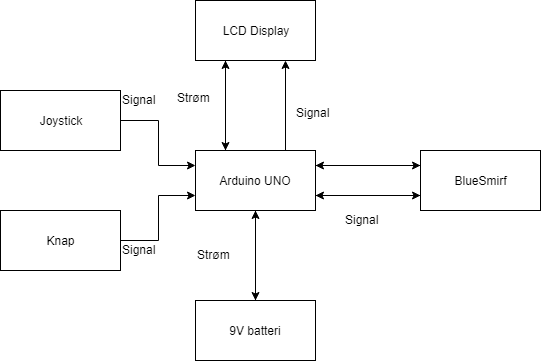
\includegraphics[scale=0.8]{Billeder/Kredsloeb2.png}
\caption{Blokdiagram af controllerens elektriske kredslob.}
\label{fig:Blokdiagram2}
\end{figure}


\begin{figure}[H]
\centering
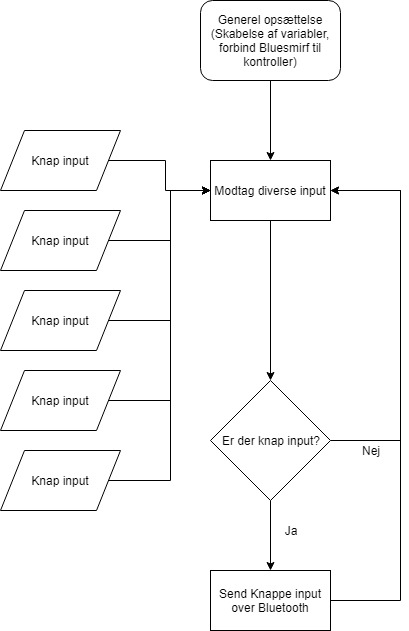
\includegraphics[scale=0.8]{Billeder/Flowchart2.jpg}
\caption{Flowdiagram af controllerens funktion.}
\label{fig:Flowdiagram2}
\end{figure}

\newpage
\textbf{Systemdele}


%Liste
\begin{itemize}
	\item Arduino UNO / Mikrocontroller
\begin{itemize}
\item På blokdiagrammet kan det ses, at Arduinoen er forbundet til næsten alle elektroniske elementer i kanontårnet. I arduinoens sted kan gruppens egen mikrocontroller print også monteres, da den har samme funktionalitet.
\end{itemize}

	\item 9V batteri
\begin{itemize}
\item Dette 9 volts batteri fungere som Arduinoens strømforsyning.
\end{itemize}

	\item Knap \#1
\begin{itemize}
\item Denne knap sender et signal til Arduinoen/Mikrocontrolleren.
\end{itemize}

	\item Knap \#2
\begin{itemize}
\item Denne knap sender et signal til Arduinoen/Mikrocontrolleren.
\end{itemize}

	\item Knap \#3
\begin{itemize}
\item Denne knap sender et signal til Arduinoen/Mikrocontrolleren.
\end{itemize}

	\item Knap \#4
\begin{itemize}
\item Denne knap sender et signal til Arduinoen/Mikrocontrolleren.
\end{itemize}

	\item Knap \#5
\begin{itemize}
\item Denne knap sender et signal til Arduinoen/Mikrocontrolleren.
\end{itemize}

	\item BlueSmirf
\begin{itemize}
\item BlueSMiRF komponenten “Silver mate” er forbundet til Arduinoen. BlueSMiRF’en sender og modtager signaler fra Arduinoen. Arduinoen fungerer som strømforsyning til BlueSMiRF’en.

\end{itemize}


\end{itemize}





\newpage
\section{Hardware}

\subsection{Stepper motor}
En stepper motor, også ofte kaldt en “stepper” er en type af elektrisk motor som kan bruges til mange forskellige ting. En af fordelene ved at bruge en stepper motor i stedet for en DC motor er, at bevægelsen med stepper motor kan gøres meget præcist i forhold til en DC motor. Dette kommer sig af navnet “stepper motor”, da motoren ikke har en “flydende” kontinuerlig bevægelse, men bevæger sig frem i trin.\\

Bevægelsen bestemmes af magnetiske poler som tændes og slukkes alt efter hvilken retning og mængde af trin der ønskes, en stepper kræver altså en eller anden form for driver, dette kan som eksempel forekomme i form af en H-bro. Trin styres af to forskudte magnetiserede tandhjul som stemmer overens med en af de to sæt magnetiske poler, disse sidder forskudt på en sådan måde at når den ene aktiveres, trækkes det nærmeste sæt tænder med modsat polaritet frem, herefter tændes den anden pol for at rykke det andet sæt tænder frem\footnote{Video og artikel om stepmotorer: \url{https://youtu.be/0qwrnUeSpYQ} og \url{https://www.instructables.com/id/How-to-use-a-Stepper-Motor/} 
}. \\

I vores kredsløb har vi brugt stepmotorer til at kontrollere retningen på vores kanontårn, en som rotere tårnet om dens centrum, og en som styre vinklen på selve geværet. 

\subsection{DC motor}
En DC motor er simpel en elektromagnetisk motor som fungerer på det samme princip som en stepmotor. Ved at kontrollere mængden og “retningen” af strømmen som løber igennem denne motor kan motoren kontrolleres til et vist punkt. I modsætning til en stepmotor er det begrænset hvor præcist en DC motor kan styres, dog har den en flydende bevægelse samt er den mere enkel i sin funktion og er derfor lettere at kontrollere.\\

I stærk kontrast til en stepmotor har en DC motor kun to mulige forbindelsespunkter. Retning er baseret på hvordan strømforsyningen er koblet til, og hastighed er baseret på den spænding som der bliver tilført. Ved kun at have to forbindelsespunkter, samt at magneterne altid er tændt på samme tid bliver motoren langt mere enkel at bruge i forhold til en stepmotor da der ikke opstår problemer med paritet mellem de forskellige magnet elementer.



\subsection{H-bro}
En H-bro bliver brugt til at ændre strømmens retning gennem et kredsløb. Ved at styre strømmen gennem fire porte kan man tænde og slukke for ønskede elementer baseret på outputs fra en arduino. I dette projekt bruger vi H-broen til at tænde for de individuelle magneter på vores stepmotorer for at skabe, og styre, rotation. At bruge en H-bro skaber også en mængde problemer, foruden problemer med opsætning og software, falder den spænding som bliver sendt til motoren med omkring 2 volt ved brug af en standard arduino H-bro (L298N\footnote{Data om standard Arduino H-bro, Underemnet: L298N \url{https://howtomechatronics.com/tutorials/arduino/arduino-dc-motor-control-tutorial-l298n-pwm-h-bridge/}}). 

Dette kan resulterer i at motoren er knap så stærk, da dennes styrke afhænger af hvor meget strøm elektromagneterne får. 


\subsection{Knapper}
I dette projekt er der blevet brugt flere knapper. Knapper kan bruges til at registrere et brugerinput. Knapper bliver ofte brugt når man skal bruge et simpelt input. F.eks. bruges knapper i dette projekt til at registrere, hvornår hardball pistolen skal skyde ud fra brugerens tryk.\\

Knapper fungerer ved at en mikrocontroller kan afmåle en spændingsforskel som knappen skaber. En ATMega328p kan afmåle disse spændingsforskelle gennem de digitale input / output. 

\subsection{Relæ}
Et relæ er en kontakt, som kan videresende strøm, hvis det aktiveres. Det bliver aktiveret ved at strømmen skaber et elektromagnetisk felt, som er stærkt nok til at lukke kontakten inde i relæet.\\

Vi bruger relæet til at tænde og slukke for skydemekanismen i airsoft-geværet ved hjælp af strømmen fra mikrocontrolleren, som tænder for relæet, der derefter lader strømmen fra geværets batteripakke gå igennem, hvilket resulterer i affyring.



\subsection{BlueSMiRF}
I dette projekt bruger vi flere bluetooth kommunikationselementer af typen “BlueSMiRF Silver”. Disse er simple, kommandobaserede kommunikationsmodemmer, som kan bruges gennem arduino. Dette gør det muligt at bruge dem i kombination med mange af de andre komponenter i vores produkt.\\

Bluetooth-kommunikation fungerer ved svage, sekvensbaserede radiosignaler mellem forskellige enheder. Dette kommer sig af, at det originalt var tiltænkt som en trådløs løsning til overførsel af data fra enheder som mobiltelefoner, som ikke har adgang til en høj spænding. Enheder inddeles i de to kategorier “slave” og “master”. Masteren er den enhed som starter kommunikationen mellem de forbundne enheder. Den bestemmer også, hvornår slaverne må sende deres signal for at holde selve kommunikationen synkron mellem slaverne og masteren\footnote{Information om Bluetooth: \url{https://www.elprocus.com/how-does-bluetooth-work/} 
}.\\

I vores projekt har vi en master forbundet til vores controller og en slave forbundet til selve tårnet, her sender masteren så de input den får gennem seriel kommunikation til slaven som er forbundet på selve tårnet. Slaven modtager et enkelt tegn baseret på et knaptryk, som den så udføre en handling ud fra, dette kunne for eksempel være at fortælle stepmotoren at den skal køre en enkelt omgang.\\


\subsection{Accelerometer}
Et accelerometer er en elektronisk komponent som kan måle sin egen tyngdeacceleration. Mange accelerometerer kan aflæse sin tyngdeacceleration på tre akser (x, y og z). \\[0.5cm]

Man kan bruge et accelerometer til at bestemme et legemes rotation i rummet.\\[0.5cm] 

I dette projekt har vi brugt et accelerometer til at bestemme hældningen på vores gevær, og den har haft til opgave at stoppe geværet fra at hæve eller sænke sig for meget ved kombineret brug af accelerometer og interrupt i kode. Ved at vurdere sin placering har accelerometeret kunne bestemme om geværet er oversteget nogle forudbestemte maksimums- og minimumsværdier for geværet hældning, og har så, baseret på disse værdier, stoppet geværet i at hæve eller sænke sig mere end hvad er tilladt.



\subsection{Spændingsregulator}
En spændingsregulator virker som en zenerdiode, der kun tillader strøm op til en bestemt spænding at løbe igennem. Zenerdioder adskiller sig fra normale dioder ved, at de ikke prøver at spærre for alt strøm, men i stedet kun spærrer for strøm, som overstiger spændingsgrænsen.\\

Vi har i projektet brugt spændingsregulatoren LM7805, da denne korrekt nedskalerer vores strømkilde (9V) til de 5V en ATMega328p må få. Mere om kredsløbet, som komponenten indgår i kan findes under afsnittet om mikrocontrollerens el-diagram.



\subsection{Mikrocontroller (ATMega328p)}

ATMega’en er en programmerbar mikrocontroller, der er standardchippen i en Arduino UNO, hvilket betyder at den kan programmeres igennem Arduino IDE’en. Mikrocontrolleren har 28 pins, hvor af 13 er digitale pins (PD\# og PB\#) og 6 kan bruge PWM (pulse width modulation). Derudover har mikrocontrolleren 8 analoge pins (PC\#), hvor PC6 også er controllerens reset-pin, samt 2 VCC, 2 GND og en reference spænding (AREF).\\


\begin{figure}[H]
\centering
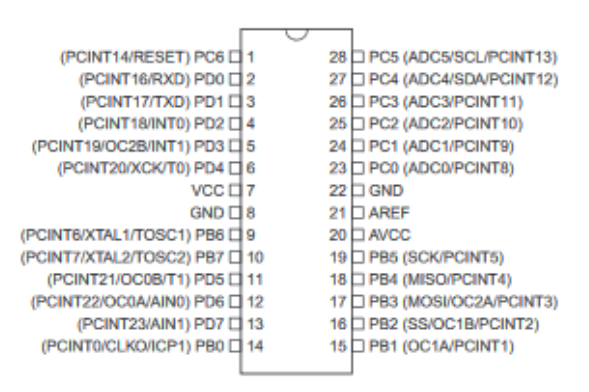
\includegraphics[scale=0.8]{Billeder/Mikrocontroller_pins.png}
\caption{Billede af ATMega328p's pin layout.}
\label{fig:ATMega_pin}
\end{figure}

Vi har i modsætning til tidligere projekter brugt en ATMega328p uden, at den sidder fast i en Arduino. Hvis denne sættes korrekt op, kan den dog udføre de samme opgaver, selvom dens programmering kompliceres ved, at den enten skal fastspændes i en Arduino hver gang, eller have en forbindelse mellem Arduino’ens TX og RX og ATMega’ens RX og TX (PD0 og PD1). Hvordan ATMega’en sættes op udenfor en Arduino kan ses under det næstkommende el-diagram afsnit.



\subsection{Krystaloscillator}
Vi bruger en 16 MHz krystaloscillator til at holde styr på ATMega’ens tidstagning. Krystallen virker ligesom en oscillator, da den bringes i stabile svingninger af strømmen fra mikrocontrolleren. Krystallens store stabilitet gør den i stand til at holde tiden ekstremt præcist, hvilket gør den ideel, hvis dele af ens kode kræver tidsstyring, som f.eks. præcise delays. \\

Mere om vores brug af krystaloscillatoren kan findes i afsnittet om mikrocontrollerprintet.

\subsection{El-diagrammer}
\subsubsection{Mikrocontrollerprint}

\begin{figure}[H]
\centering
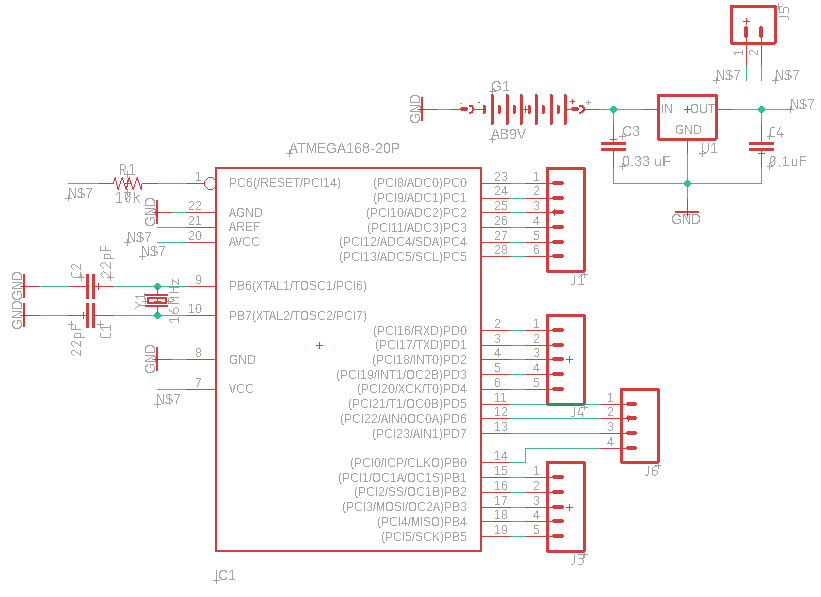
\includegraphics[scale=0.8, angle=90]{Billeder/El-diagram.PNG}
\caption{El-diagram over mikrocontrollerprint.}
\label{fig:El_diagram_mikro}
\end{figure}

Selve mikrocontrollerprintet består af 2 forbundne kredsløb. Det første er selve ATMEGA’en, som er udstyret med en krystaloscillator (Y1 på figur \ref{fig:El_diagram_mikro}), som er yderligere forklaret under hardware-afsnittet. Der er forbundet 2 kapacitorer mellem krystaloscillatoren og GND for at forbedre strømmens stabilitet. Krystaloscillatorens størrelse (16 MHz), samt kapacitorernes størrelse (22 pF) er baseret på ATMega’ens datablad, hvor disse er foreslået\footnote{ATMega datablad, afsnit 9.4: \url{http://ww1.microchip.com/downloads/en/DeviceDoc/ATmega48A-PA-88A-PA-168A-PA-328-P-DS-DS40002061A.pdf}}.\\

Derudover er der lavet huller til alle ATMega’ens resterende pins, så de kan bruges frit, ligesom på en Arduino. Ligesom det kan ses på el-diagrammet er ATMega’ens 2 GND pins forbundet til pladens GND og de to VCC pins, samt AREF er forbundet til den regulerede 5 volts kilde. Arduino’ens reset-pin er forbundet til 5 volts kilden igennem en 10 kΩ resistens, så spændingen forhindrer ATMEGA’en i at genstarte af sig selv.\\

Det andet, mindre kredsløb på mikrocontrollerprintet er spædningsregulatoren, som kan ses øverst til højre på figur \ref{fig:El_diagram_mikro}. Denne er tilstede, da mikrocontrolleren ikke må få mere end 5V. De to kapacitorer, som er tilsluttet selve spændingsregulatoren sørger for bedre stabilitet og er tilføjet, da dette var opfordret i komponentens datablad, hvis man vil have et konstant 5V output\footnote{M7805 datablad, side 7: \url{https://www.sparkfun.com/datasheets/Components/LM7805.pdf}}.

\subsection{PCB-layout}

\begin{figure}[H]
\centering
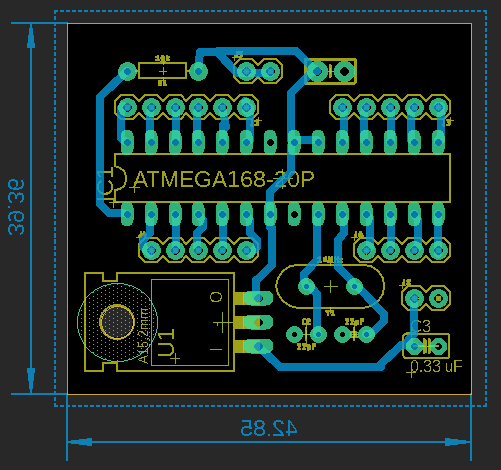
\includegraphics[scale=0.8]{Billeder/PCB_uden_kobber.PNG}
\caption{PCB-layout med angivede mål. Uden kobber på pladen.}
\label{fig:PCB}
\end{figure}

Layout’et er lavet i Eagle ud fra el-diagrammet på figur \ref{fig:PCB}. Alle komponenterne er placeret, så de fylder så lidt som muligt, men samtidig er mulige at lodde præcist i hånden. Som det kan ses på figur \ref{fig:PCB}, har vores mikrocontrollerprint dimensionerne: 42,85 x 39,36 mm.

\begin{figure}[H]
\centering
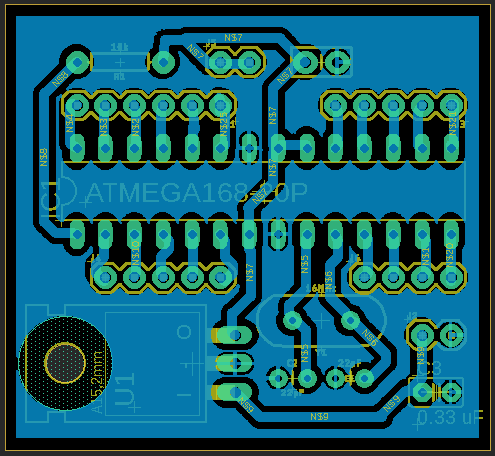
\includegraphics[scale=0.8]{Billeder/PCB_med_kobber.PNG}
\caption{PCB med kobber (GND) på pladen.}
\label{fig:PCB_kobber}
\end{figure}

Som illustreret på figur \ref{fig:PCB_kobber}, er der én samlet GND på pladen, som alt er forbundet til. Dette sparer meget plads, hvis sammenlignet med en løsning, hvor f.eks. en Arduino skulle have sin egen separate GND. Hvis man tænker på at hele mikrocontrollerprintet, egentlig bare er en simpel Arduino, giver det også mening at den skal være så lille som muligt, da dette er den “hjemmelavede” Arduinos største fordel, hvis sammenlignet med en standard Arduino UNO. En Arduino UNO vil f.eks. ikke kunne passe ind i en kompakt controller, mens dette mikrocontrollerprint ville kunne pakkes meget kompakt med dets minimale dimensioner.







\newpage
\section{Software}
I dette afsnit gennemgåes de forskellig dele af softwaren ved brug af flowcharts og psedokode.

\subsection{Generelt}
I dette projekt har vi skulle skrive en form for “OS” (Operating System) til vores kanontårn. Denne OS skal selvfølgelig stemme overens med opgavens krav. Den skal altså kunne bruges på et arduino chipset, samt være i stand til at afbryde handlinger baseret på input fra en controller-enhed.

\subsection{IDE og sprog}
Som sagt er der i projektet skrevet et program til et Arduino chipset. Selve programmet skal altså skrives i et sprog som Arduinoen kan forstå. I dette tilfælde er der skrevet i det Arduino dedikerede sprog, også kaldet Wire, som er en forgrening af de meget udbredte sprog “C” og “C++”\footnote{\url{ https://www.arduino.cc/en/Main/FAQ}}. Der er i projektet også brugt Arduinos egen basis IDE (Integrated Development Environment) da selve funktionerne og fejlfinding i dette projekt ikke har været problematisk nok til at kunne understøtte at bruge tid på at finde en udvidelse eller helt nyt udviklingsmiljø.

\subsection{Indsamling af viden om Arduino software}
I projektet har vi skulle bruge mange nye komponenter for at kunne opfylde de stillede krav. Dette har resulteret i, at det har været nødvendigt at søge ny information. Basis-principper vedrørende de nye komponenter er primært fundet fra siden “Sparkfun”\footnote{\url{https://learn.sparkfun.com/tutorials/using-the-BlueSMiRF/all }}, som har mange gode eksempler på både brug af komponenter og de mange forskellige måde som disse kan kobles til, og kommunikeres med gennem Arduino\footnote{Problemløsning med knapper:\url{https://www.arduino.cc/en/Tutorial/Button
}}. Udover denne hjemmeside har spørgsmålssegmentet på Arduinos egen hjemmeside ofte givet gode råd og har kunnet besvare spørgsmål med deres store forum.


\subsection{Program flow}
\begin{figure}[H]
\centering
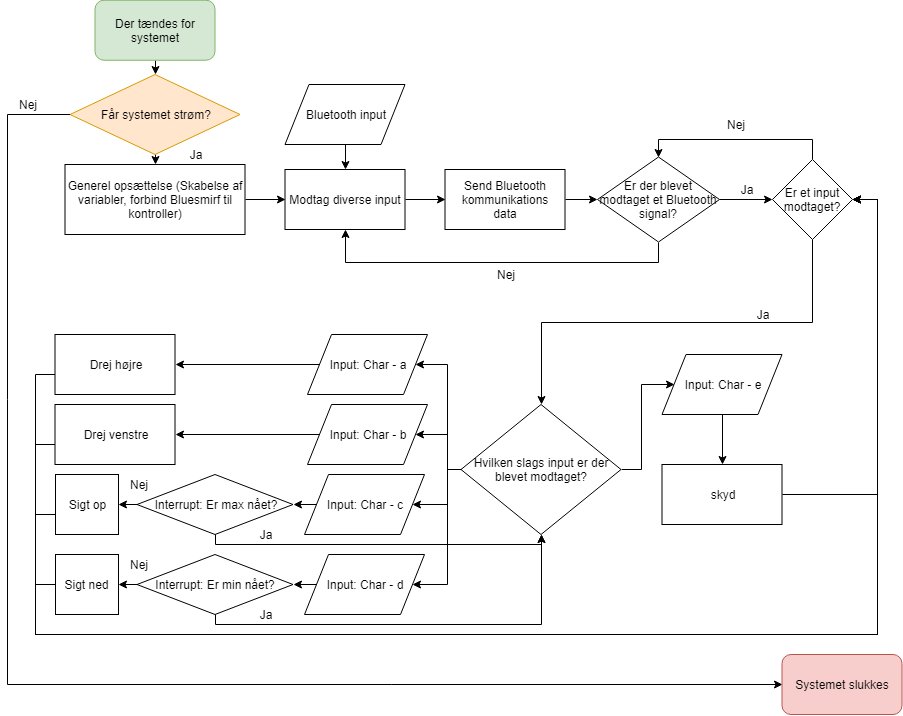
\includegraphics[scale=0.6,angle= 90]{Billeder/ProgramFlowchart.png}
\caption{Flowchart over softwarens logik.}
\label{fig:ProgramFlow}
\end{figure}

\subsection{Psedokode}
\subsubsection{Controller}
Oenskede biblioteker inkluderers, her bliver biblioteket “SoftwareSerial” inkluderet da dette skal bruges til seriel kommunikation mellem de to BlueSMiRF silver mates.\\

Foerst opsaettes Pins og globale vaerdier:\\
	//Nedenstaaende er pins som bruges til knapper\\
	KnapVenstre = 4\\
	KnapHojre = 5\\
	KnapOp = 6\\
	KnapNed = 7\\
	KnapSkyd = 8\\
	//Variabler til registreing af knaptryk\\
	KnapStateVenstre = 0\\
	KnapStateHojre = 0\\
	KnapStateOp = 0\\
	KnapStateNed = 0\\
	KnapStateSkyd = 0\\
	//Bluetooth pins til kommunikation oprettes\\
	BluetoothTx = 2\\
	BluetoothRx = 3\\

Herefter opsaettes “Void setup” hvor pins defineres til inten OUTPUT eller INPUT, og bluetooth kommonikations paabegyndes.\\
	Knap pins saettes til input\\
	Serial port startes ved standard baudrate paa 9600\\
	Bluetooth opstartes ved standard baudrate paa 115200\\
	Kommandosekvens paabegyndes.\\
	Naar kommandosekvensen har koert saettes baudraten ned fra 115200 til 9600\\ for ikke\\
	At skabe problemer med arduino kommunikation.\\
	Print “Ended Setup”\\

Der oprettes en boolsk vaerdi til at vurdere om kommandosekvens til opretelse af denne bluetoothenhed som master har koert.\\

Void loop:\\
	Der oprettes fem led i et elif statement til at sende fem kommando karaktere:\\
	Hvis knaptryk(a,b,c,d eller e):\\
		Send a,b,c,d eller e gennem bluetooth (korresponderende bogstav til knaptryk)\\
		Vent 250 millisekunder.\\
	Hvis bluetooth er tilgaengelig:\\
printes alle karaktere som er blevet sendt eller modtaget paa denne enheds serial  monitor.\\
	Ellers:\\
 printes der ikke noget.\\
 

\subsubsection{Turret}
Oenskede biblioteker inkluderers, her bliver biblioteket “SoftwareSerial” inkluderet da dette skal bruges til seriel kommunikation mellem de to BlueSMiRF silver mates.\\

Først opsaettes Pins og globale vaerdier:\\
	//Nedenstaaende er pins som bruges til at styre diverse dele af systemet:\\
	Hojre = 8 // 8 og 9 er til rotationsmotor\\
	venstre = 9\\
	Op = 10  // 10 og 11 er til at panorere op eller ned\\
	Ned = 11\\
	Skyd = 12 // pin 12 er til at skyde med\\
	LedPin = 13 // Til interrupt\\
	
	Volatile int state = LOW // Kontrol af led i interrupt, dette state er som standard LOW\\

	//Bluetooth pins til kommunikation oprettes\\
	BluetoothTx = 3\\
	BluetoothRx = 4\\

Herefter opsaettes “Void setup” hvor pins defineres til inten OUTPUT eller INPUT, og bluetooth kommonikations påbegyndes.\\
	Foerst startes seriel kommunikation ved en baudrate på 115200 som standard.\\
	Herefter initieres kommandosekvens.\\
	En kort pause for at sikre at mate’n sender cmd.\\
	Pins til kontrol saettes alle til OUTPUT.\\
Serial kommunikation startes ved standard baudrate på 9600 da 115200 kan vaere for  hurtigt til stabil kommunikation.\\
	Pins til motor og skud kontrol oprettes som OUTPUT.\\
	Interrupt oprettes til funktionen “blink” ud fra parameteren “state” og en aendring i state.\\
	Led Pin saettes til OUTPUT\\
$Interrupt standard pin INT0 saettes til “INPUT_PULLUP” som hiver interrupt segmentet frem i “stack”.$\\

Interrupt funktionen “Blink” oprettes:\\
	State = !state // her sker en aendring hvis et interrupt forekommer.\\

Void loop:\\
	Først sikres det at alle OUTPUT pins er LOW\\
	Hvis bluetooth er tilgaengelig:\\
		Opret switch statement med en case for hvert kommando tegn fra controleren,\\
		Altså a, b, c, d og e, som henholdsvis kontrolere en bestemt handling.\\


\subsection{Programbeskrivelse/gennemgang}
Selve Kanontårnets og controllerens OS er lavet i arduino til brug på både arduino UNO chipsæt og gruppens egen mikrocontroller. programmet indsamler data fra en sensor og flere forskellige knapper og bruger disse data til at bestemme tårnets handling.Hvis kanontårnet modtager en værdi baseret på et knaptryk fra controlleren vil tårnet udføre en af disse handlinger: Drej til højre, drej til venstre, panorer op, panorer ned og skyd. Hvis kanontårnet kommer til en max eller min værdi for geværets “hældning” registrere accelerometeret dette og bruger interrupt til at stoppe geværet fra at hæve eller sænke sig. Hvis ikke kanontårnet får noget input, eller ikke får noget bluetooth signal vil tårnet forholde sig í ro.







\newpage
\section{Ikke elektroniske dele}
I dette afsnit gennemgås produktionen af de ikke-elektriske dele af produktet og mikrocontrollerprintet.

\subsection{Production af kanontårn}
Hele den fjernstyret kanon er holdt sammen af et kanontårn. Dette “skelet” er lavet af MDF (Medium Density Fiberboards) plader. Der er i alt fire forskellige plader. To af pladerne bruges som bunde, som skaber rotation om z-aksen. De sidste to plader fungerer som arme, som griber rundt om våbnet. Disse arme tillader rotation om x/y-aksen. \\

\begin{figure}[H]
\centering
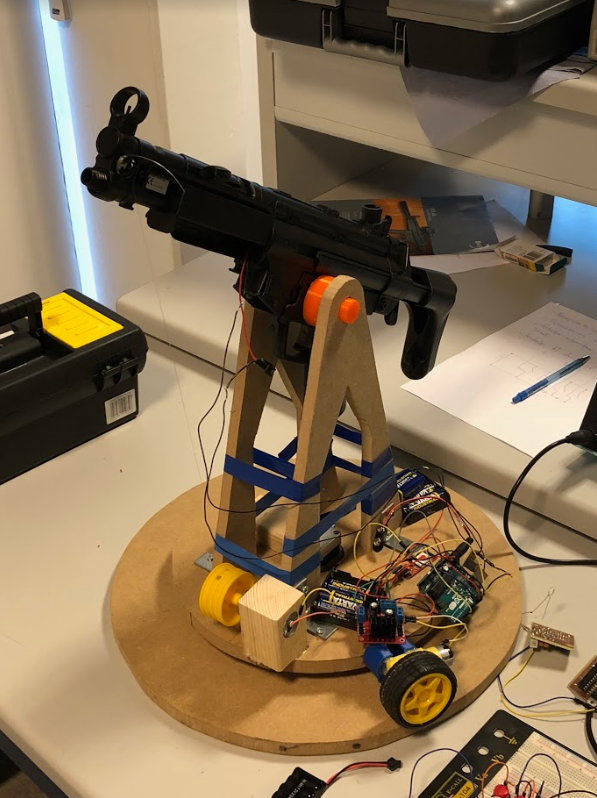
\includegraphics[scale=0.4]{Billeder/Kanontarn.PNG}
\caption{Det faerdiglavet produkt hvor skelettet kan ses.}
\label{fig:Kanontarn_faerdig}
\end{figure}

De fire plader er designet på sådanne måde, at de skal veje så lidt som muligt. De er blevet designet på sådanne måde, da motoren som sørger for rotation om z-aksen er mere effektiv, jo mindre vægt den skal flytte. Derudover er skelettet designet rundt om hardball-våbnet BT5\footnote{\url{https://www.legbilligt.dk/shop/14-el-gevaer---billige-softguns/238-bt---bt5-a5-kompletsaet/}} , som monterers på skelettet. 

\subsection{Production af 3D print}
Ud over de fire MDF plader er der også blevet produceret 3D-printet komponenter til kanontårnet. Alle de 3D-printede komponenter er lavet i Autodesk Fusion 360. \\

Alle de 3D-printede komponenter er designet til at hjælpe motoren med at roterer. \\

\begin{figure}[H]
\centering
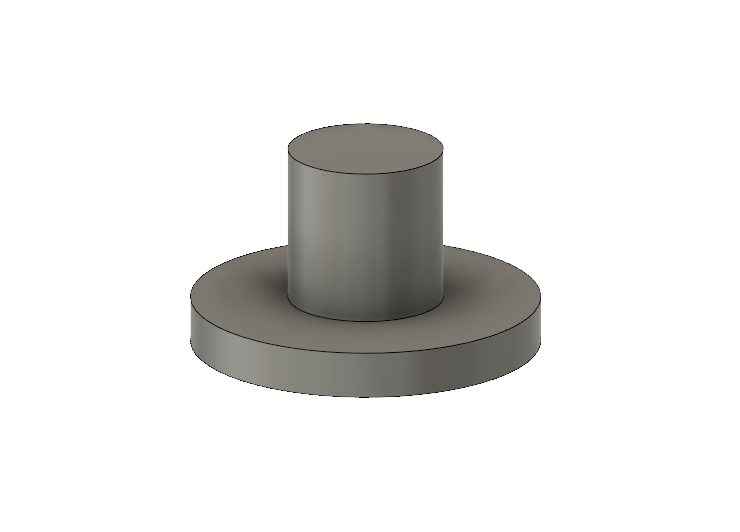
\includegraphics[scale=0.4]{Billeder/3D_print_1.PNG}
\caption{3D-print som hjaelper med x/y-rotation.}
\label{fig:3D_print_1}
\end{figure}

Dette komponent kan findes på begge sider af den monteret hardball pistol. Dette komponent hjælper med rotationen om x/y-aksen. \\

\begin{figure}[H]
\centering
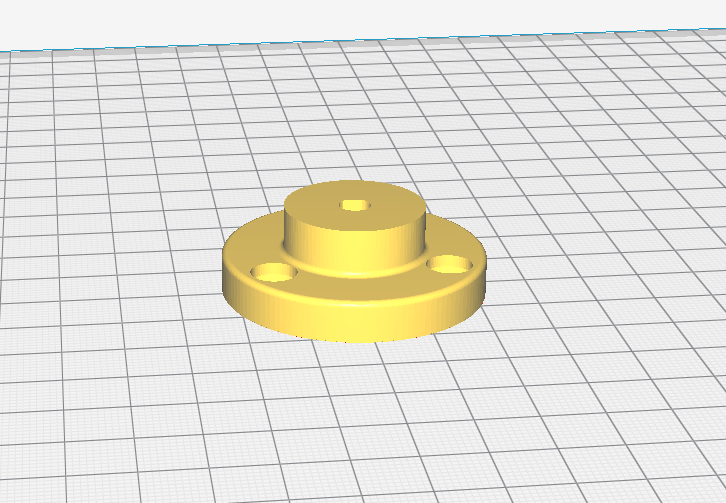
\includegraphics[scale=0.4]{Billeder/3D_print_2.PNG}
\caption{3D-print som hjaelper med z-rotation.}
\label{fig:3D_print_2}
\end{figure}

Dette komponent kan findes mellem de to MDF bundplader og hjælper med rotation om z-aksen.  \\

\subsection{Production af mikrocontrollerprint}

\begin{figure}[H]
\centering
\includegraphics[scale=0.4]{Billeder/Printpapir.jpg}
\caption{ Det gennemsigtige papir, som blev brugt til maalrettet belysning af kobberpladen.}
\label{fig:mikrocontrollerprint}
\end{figure}


Printet er anmærket ved at belyse en kobberplade dækket med lysfølsomt materiale gennem et gennemsigtigt papir, hvor kredsløbet er anmærket (se figur \ref{fig:mikrocontrollerprint}).\\


Printet er herefter blevet nedsænket i en svag natriumhydroxidopløsning, der kun fjerner den lysfølsomme belægning fra det belyste område. Dette gør, at når printet herefter nedsænkes i et syrebad, vil kun det kobber, hvorfra det ekstra lysfølsomme lag er opløst, blive ætset væk. Når dette er sket placeres printet i en stærkere natriumhydroxidopløsning, så resten af det lysfølsomme lag forsvinder. 








\newpage
\section{Aftestning}

\subsection{Test med præfabrikeret H-bro (L289N)}

\begin{figure}[H]
\centering
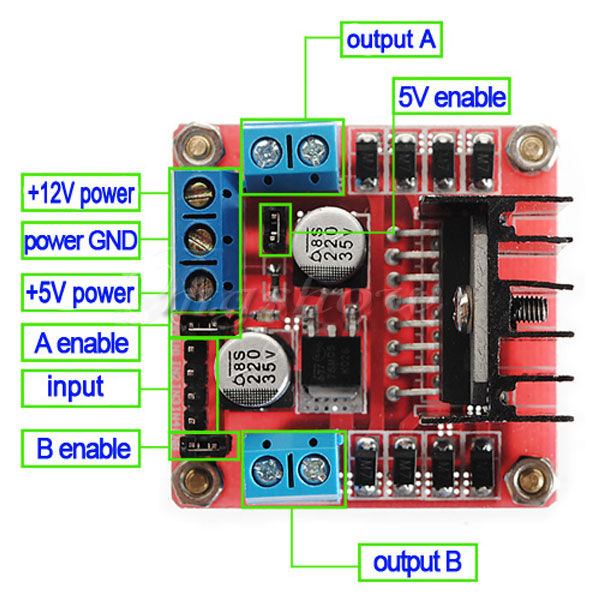
\includegraphics[scale=0.4]{Billeder/H-bro.jpg}
\caption{ En forudproduceret H-bro.}
\label{fig:mikrocontrollerprint}
\end{figure}

Til aftestning har gruppen gjort brug af en L289N-enhed. Dette er en færdig H-bro som bruges til at controllere retning og omdrejninger på en stepmotor/DC motor. Denne enhed har op til 6 input pins samt 1-2 pins til strømforsyning. Den ene af disse pins kan laves om til et output for en lav strømforsyning, for eksempel til en arduino, hvis der er forbundet en strømforsyning til den anden port på +12V. Den sidste pin skal forbindes til ground.

\subsection{Test af knapper}

Som en del af vores produkt har vi produceret en trådløs controller til at styre vores tårn med. denne controller fungere ved input gennem fem knapper, en til hver kommando. I vores forløb har vi prøvet flere forskellige opsætning af knapper, med hver deres modstand, en enkelt, og brug af forskellige ledninger. Det er blevet bestemt ud fra forsøg at et sådant knapsystem fungere bedst hvis alle knapper har deres egen modstand inden de går til jord, samt at mere ukonventionel opsætning og placering generelt skaber flere problemer end de løser. Ved brug af samme placering som på moderne spillemaskine-controller opstod der signalforstyrrelser som ikke var til at fjerne, og ved en enkelt stor modstand blev signalerne fra knapperne sjældent stoppet når de var blevet trykket ned.\\

I sidste ende har vi valgt at lave en række med fem knapper med hver deres modstand og en kombineret forbindelse til jord.

\subsection{Aftestning af mikrocontroller og mikrocontrollerprint}
Inden arbejdet med selve mikrocontrollerprintet begyndtes, testede vi kredsløbet på et fjumrebræt for at sikre, at det virkede som tiltænkt inden produktionen af printet startedes, da en fejl i printets design tager meget længere tid at fikse, hvis den opdages for sent.

\begin{figure}[H]
\centering
\includegraphics[scale=0.4]{Billeder/Fjumrebraet.jpg}
\caption{  Foerste test af mikrocontrollerprintet på et fjumrebraet. Oeverst til hoejre kan spaendingsregulatoren ses, mens ATMega’en og de tilhoerende forbindelser er til venstre.}
\label{fig:fjumrebraet}
\end{figure}

Efter at testen, som gik ud på at få en lysdiode til at stige og falde i lysstyrke, virkede på fjumrebrættet, kunne selve produktionen af mikrocontrollerprintet begynde. Da printet var blevet færdigproduceret testede vi alle forbindelser på det, for at opdage eventuelle produktionsfejl.

\begin{figure}[H]
\centering
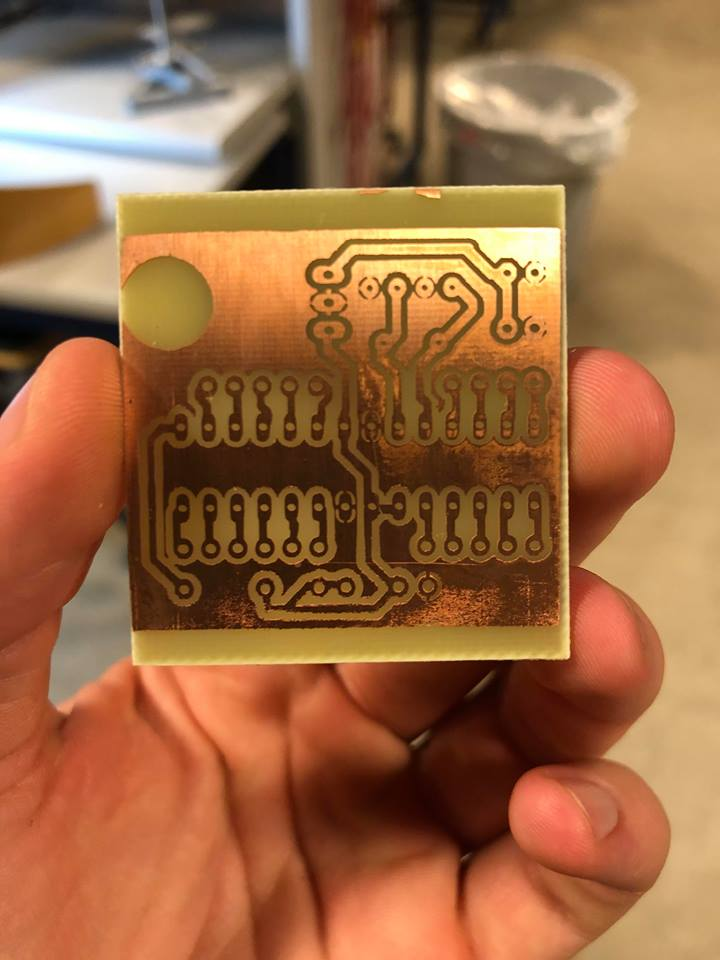
\includegraphics[scale=0.4]{Billeder/print.jpg}
\caption{ Kobberforbindelserne på det nylavede mikrocontrollerprint.}
\label{fig:print_test}
\end{figure}

Det første print vi lavede havde en fejl, da det var blevet spejlvendt under produktionen, hvilket gjorde at alle de “ikke-spejlbare” komponenter (ATMega328p og LM7805) skulle loddes fast på den modsatte side af printet, end hvor man normalt gør det. Der skulle altså loddes under selve komponenten istedet for på den anden side af printet. Det kom dog til at virke, selvom det var betydeligt mere vanskeligt loddearbejde end normalt.


\begin{figure}[H]
\centering
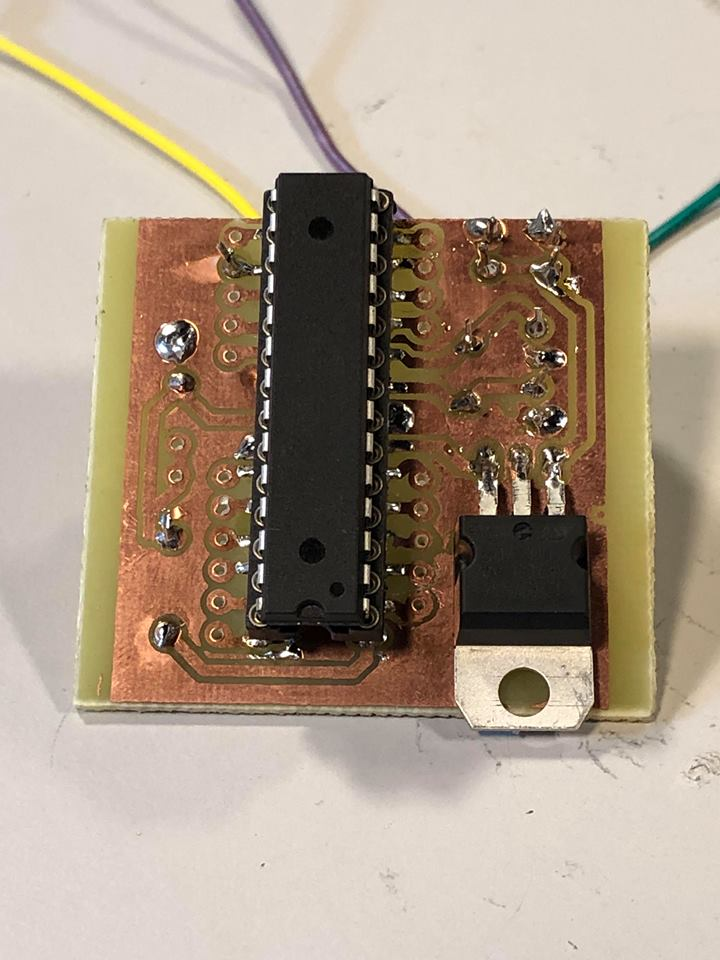
\includegraphics[scale=0.4]{Billeder/spejlvendtprint.jpg}
\caption{ Det færdiglavede og fuldt funktionelle spejlvendte print.}
\label{fig:print_test}
\end{figure}

Vi testede printets funktionalitet ved brug af den samme test, som før printarbejdet blev påbegyndt, da denne derfor var bevidst til at skulle virke. Vi lavede også et andet print, da vi ikke var sikre på om den spejlvendte kunne loddes korrekt, men denne havde flere produktionsfejl, da den manglede de anmærkede kobberbaner flere steder. Dette førte til, at den blev næsten umulig at lodde korrekt og skulle kasseres.

\begin{figure}[H]
\centering
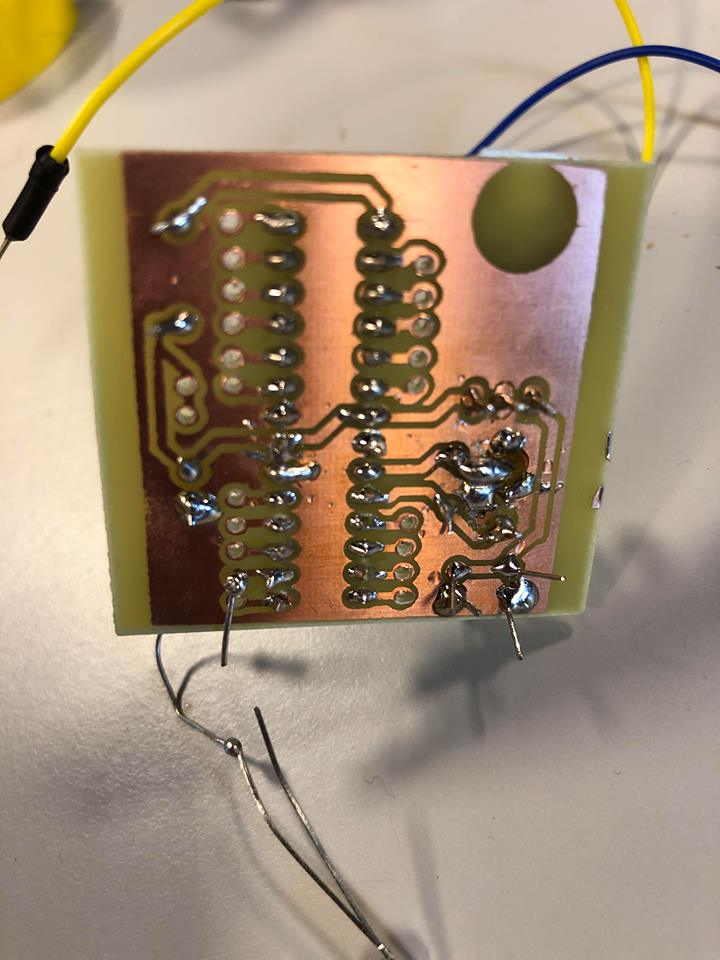
\includegraphics[scale=0.4]{Billeder/fejlprint.jpg}
\caption{ Loddefejlen nederst til hoejre på fejlprintet skyldes de manglende/beskadigede kobberbaner.}
\label{fig:print_test}
\end{figure}




\subsection{Problemer under udviklingen af produktet }
\subsubsection{Problem \#1 - Stepper motor vs. DC motor}
I den største del af projektet har vi i gruppen forsøgt at gøre brug af to stærke stepper motorer til at hæve og sænke geværet samt dreje selve platformen. Vi har dog haft store problemer med bare at få disse motorer til at lave simple rotationer. Det første problem vi stødte på var ikke at få selve motoren til at køre, det var at dem vi havde fundet var for svage og havde en for lav trækkraft. Disse blev så skiftet ud med to større motorer, som hver har en trækkraft på cirka 10 kg. Disse havde dog også et meget stort problem, de virkede kun halvdelen af tiden, den anden halvdel vibrerede de bare. Problemet opstod formentlig i enten koden eller selve kredsløbet, men begge disse er blevet ændret på alle tænkelige måder for at løse dette problem. I sidste ende har vi skiftet begge stepper motorer ud med DC motor, disse er både lettere at bruge, samt har de ingen af de samme problemer som stepper motorne havde. Der er dog et argument for at selve tårnets bevægelse ikke er lige så præcis, dog var selve ideen at den skulle dreje efter hvor længe man holder en bestemt knap inde, så selve den endelige bevægelse bliver ikke påvirket af dette skift af motoren.

\subsubsection{Problem \#2 - Flydende kommunikation}
I den sidste del af projektet har vi haft problemer med flydende bevægelser ud fra vores givne kommandoer, i et normalt program uden trådløs kommunikation ville man kunne opnå en “flydende overgang” fra kommando til handling ved at definere det ud fra et HIGH/LOW state, dette er dog ikke tilfældet her. Da man er nødt til at sende information som pakker er der ikke mulighed for at sende et kontinuerligt signal som kan ændre sig på samme måde som et HIGH/LOW state. For at skabe en flydende overgang skal den “pause” altså det delay, som er mellem hver kommando og udførelsen af en handling passe sammen, hvis der går længere tid mellem handlinger end mellem kommandoer ville dette resultere i at man ville kunne “indhente” den del af hardware som udføre handlingerne og endda overhale den, så den udføre handlinger, selvom man ikke trykker noget på det tidspunkt. Hvis man derimod har kortere mellem handlinger end mellem kommandoer ville det se ud som om at der er et “input lag” hvilket der i princippet også er. De to skal altså stemmer overens, man stadigt ikke ske så hurtigt at programmet og de mere mekaniske dele af hardware ikke kan følge med.\\

I disse to stykker kode ses de to tider som skal stemmer overens: 

\begin{lstlisting}[style=CStyle]
//Turret.ino

if(bluetooth.available()) //Hvis der er kommunikation med bluetooth, start switch
	switch ((char)bluetooth.read()){
		case 'a': //Hvis turret har modtaget char: a, drej til venstre i 250ms
			digitalWrite(R, LOW);
			digitalWrite(L, HIGH);
			digitalWrite(LodPin, statc);
			delay(250);
			serial.println("a");
			delay(1);
			break;	
			
\end{lstlisting}

\begin{lstlisting}[style=CStyle]
//Controller.ino

if(buttonStateLeft == HIGH){
	bluetooth.print((char) 'a');
	serial.println("a");
	delay(250);
}

\end{lstlisting}


I en længere periode var begge et helt sekund, dette resulterede i ringe kontrol og en fornemmelse af “lag” hvis man sænker tiden for handlingen uden at sænke for kommandoen vil der forekomme bevægelser i hak. 250 ms til hver lader til at være et sweet spot hvor der er en god følelse af kontrol, men også et punkt hvor motoren og H-broen kan nå at reagere på input fra Arduino.









\newpage
\section{Konklusion}
\newpage

\section{Litteraturliste}
\emph{Teknisk Matematik} af Preben Madsen, 4. Udgave. \\[0.5cm]
\emph{Orbit B} af Per Holck, Jens Kraaer og Birgitte Merci Lund. \\[0.5cm]
\url{http://www.matematikfysik.dk/fys/noter_tillaeg/tillaeg_det_skraa_kast_uden_luftmodstand.pdf} af \url{http://www.matematikfysik.dk}. Senest læst den 19/12/2018.\\[0.5cm]
\url{http://www.matematiksider.dk/projekter/skraakast.pdf} af \url{http://www.matematiksider.dk}. Senest læst den 19/12/2018







\newpage

\section*{Bilag}




\end{document}
